\documentclass[a4paper,12pt]{exam}
	\usepackage{graphicx}
	\usepackage[utf8]{inputenc}
	\usepackage[T1]{fontenc}
	\usepackage{listings}
	\usepackage{color}
	\usepackage{amsmath}
	\usepackage{enumerate}
	\usepackage{caption}
	\usepackage{subcaption}
	\usepackage{hyperref}
	\usepackage{footnote}
	\definecolor{dkgreen}{rgb}{0,0.6,0}
	\definecolor{gray}{rgb}{0.5,0.5,0.5}
	\definecolor{mauve}{rgb}{0.58,0,0.82}

	\lstset{frame=tb,
	  language=Python,
	  aboveskip=3mm,
	  belowskip=3mm,
	  showstringspaces=false,
	  columns=flexible,
	  basicstyle={\small\ttfamily},
	  numbers=none,
	  numberstyle=\tiny\color{gray},
	  keywordstyle=\color{blue},
	  commentstyle=\color{dkgreen},
	  stringstyle=\color{mauve},
	  breaklines=true,
	  breakatwhitespace=true
	  tabsize=3
	}

\begin{document}
	\begingroup 
	  \bf \Large Mecânica Clássica I\\
	  \indent \normalsize André Del Bianco Giuffrida
	\endgroup
	\\ \quad
	\\
	Segundo Kepler: \\
	\textit{ Os quadrados dos períodos de revolucão ($T$) são proporcionais aos cubos das distâncias médias ($a$) do Sol aos planetas. $T^2=ka^3$, onde $k$ é uma constante de proporcionalidade.}\\
	\\
	Partindo dos dados:
	
	\begin {table}[h]
	Orbital Data
	\centering
		\[
		\begin{tabular}[c]{l*{9}{c}r}
			Name & Distance (km) & Period (days) & Incl & Eccen\\
			\hline
			Mercury &     57910   & 87.97    & 7.00  & 0.21 & \\
			Venus   &     108200  & 224.70   & 3.39  & 0.01 & \\
			Earth   &     149600  & 365.26   & 0.00  & 0.02 & \\
			Mars    &     227940  & 686.98   & 1.85  & 0.09 & \\
			Jupiter &     778330  & 4332.71  & 1.31  & 0.05 & \\
			Saturn  &     1429400 & 10759.50 & 2.49  & 0.06 & \\
			Uranus  &     2870990 & 30685.00 & 0.77  & 0.05 & \\
			Neptune &     4504300 & 60190.00 & 1.77  & 0.01 & \\
		\end{tabular}
		\]
	\caption{Fonte: \href{http://nineplanets.org/data.html}{http://nineplanets.org/data.html}}
	\end{table}
		
	Para Verificar se a afirmação de kepler é precisa foi utilizado o seguinte racioncínio,\\
	\[ \frac{T_{i}^2}{a_{i}^3} - \frac{T_{j}^2}{a_{j}^3} = \pm E_{ij} \] 
	Onde $E_{ij}$ é o erro encontrado ao calcular para os planetas $i$ e $j$, a matriz gerada pelos elementos $| E_{ij} |$ é uma matriz triangular, é tomado o módulo pois 
	o erro pode estar acima ou abaixo do valor de $k$ porém não agrega nenhuma nova informação, apenas que uma razão é maior que a outra, por isso o uso do módulo do Erro.\\
	\begin{figure}[h]
		\centering
		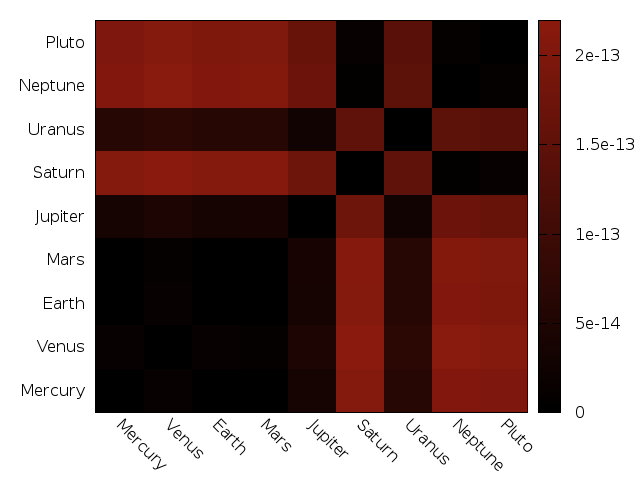
\includegraphics[scale=0.34]{8o0.png}
		\caption{ Erro $E_{ij}$ na teoria de Kepler vs dados medidos \\ para os Planetas}
	\end{figure}

	Podemos notar que o erro é da ordem de $10^{-13}$ o que é muito bom de acordo com a incerteza das medidas, porém 9 planetas são poucos dados para validar uma relação tão importante.
	Se a relação de Kepler vale para o sol, deve valer para outros astros também.
	
	Então podemos utilizar todos os dados encontrados para a Distância da órbita e o Periodo de cada astro.
	e assim obtemos a seguinte figura:
	
	\begin{figure}[h]
		\centering
		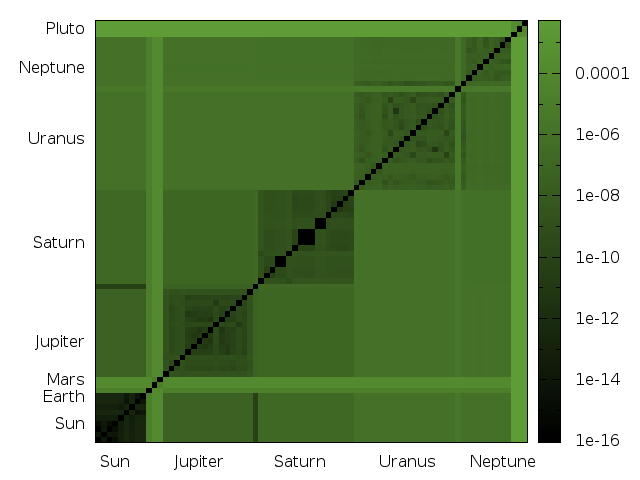
\includegraphics[scale=0.6]{8o1.png}
		\caption{ Erro $E_{ij}$ cada linha é um planeta ou satelite natural, os nomes são os astros que os satelites orbitam}
	\end{figure}
	
	Agora notamos que a precisão ainda é boa porém é melhor quando trabalhado com astros massivos, ou quando a distância entre os astros comparados é pequena, ou seja, ainda resta algo na constante de kepler $k$ que dependa da massa, e isso vai ser definido por Newton com $\frac{R^3}{T^2} = \frac{GM}{4 \pi^2}$
	
	
	\end{document}
